\section{Comparison and Evaluation}
\label{sec:evaluation}
Using the analysis of conventional and deep learning methods in action recognition, this section provides a comparison and evaluation of the presented methods.
Results of deep learning approaches, which were reviewed in this report, are given in the following table \ref{tab:deep_results}.

\begin{minipage}[b]{.03\linewidth}
\setstretch{1.25}
\scriptsize
\cite{ji_3d_2013}\\
\cite{baccouche_sequential_2011}\\
\cite{karpathy_large-scale_2014}\\
\cite{tran_learning_2015}\\
\cite{varol_long-term_2016}\\
\cite{simonyan_two-stream_2014}\\
\cite{ng_beyond_2015}\\
\cite{wang_towards_2015}\\
\cite{feichtenhofer_convolutional_2016}\\
\cite{wang_action_2015}\\
\cite{srivastava_unsupervised_2015}
\cite{palasek_action_2016}
\cite{misra_shuffle_2016}
\\\\
\end{minipage}
\begin{minipage}[b]{.96\linewidth}
\begin{table}[H]
    \centering
    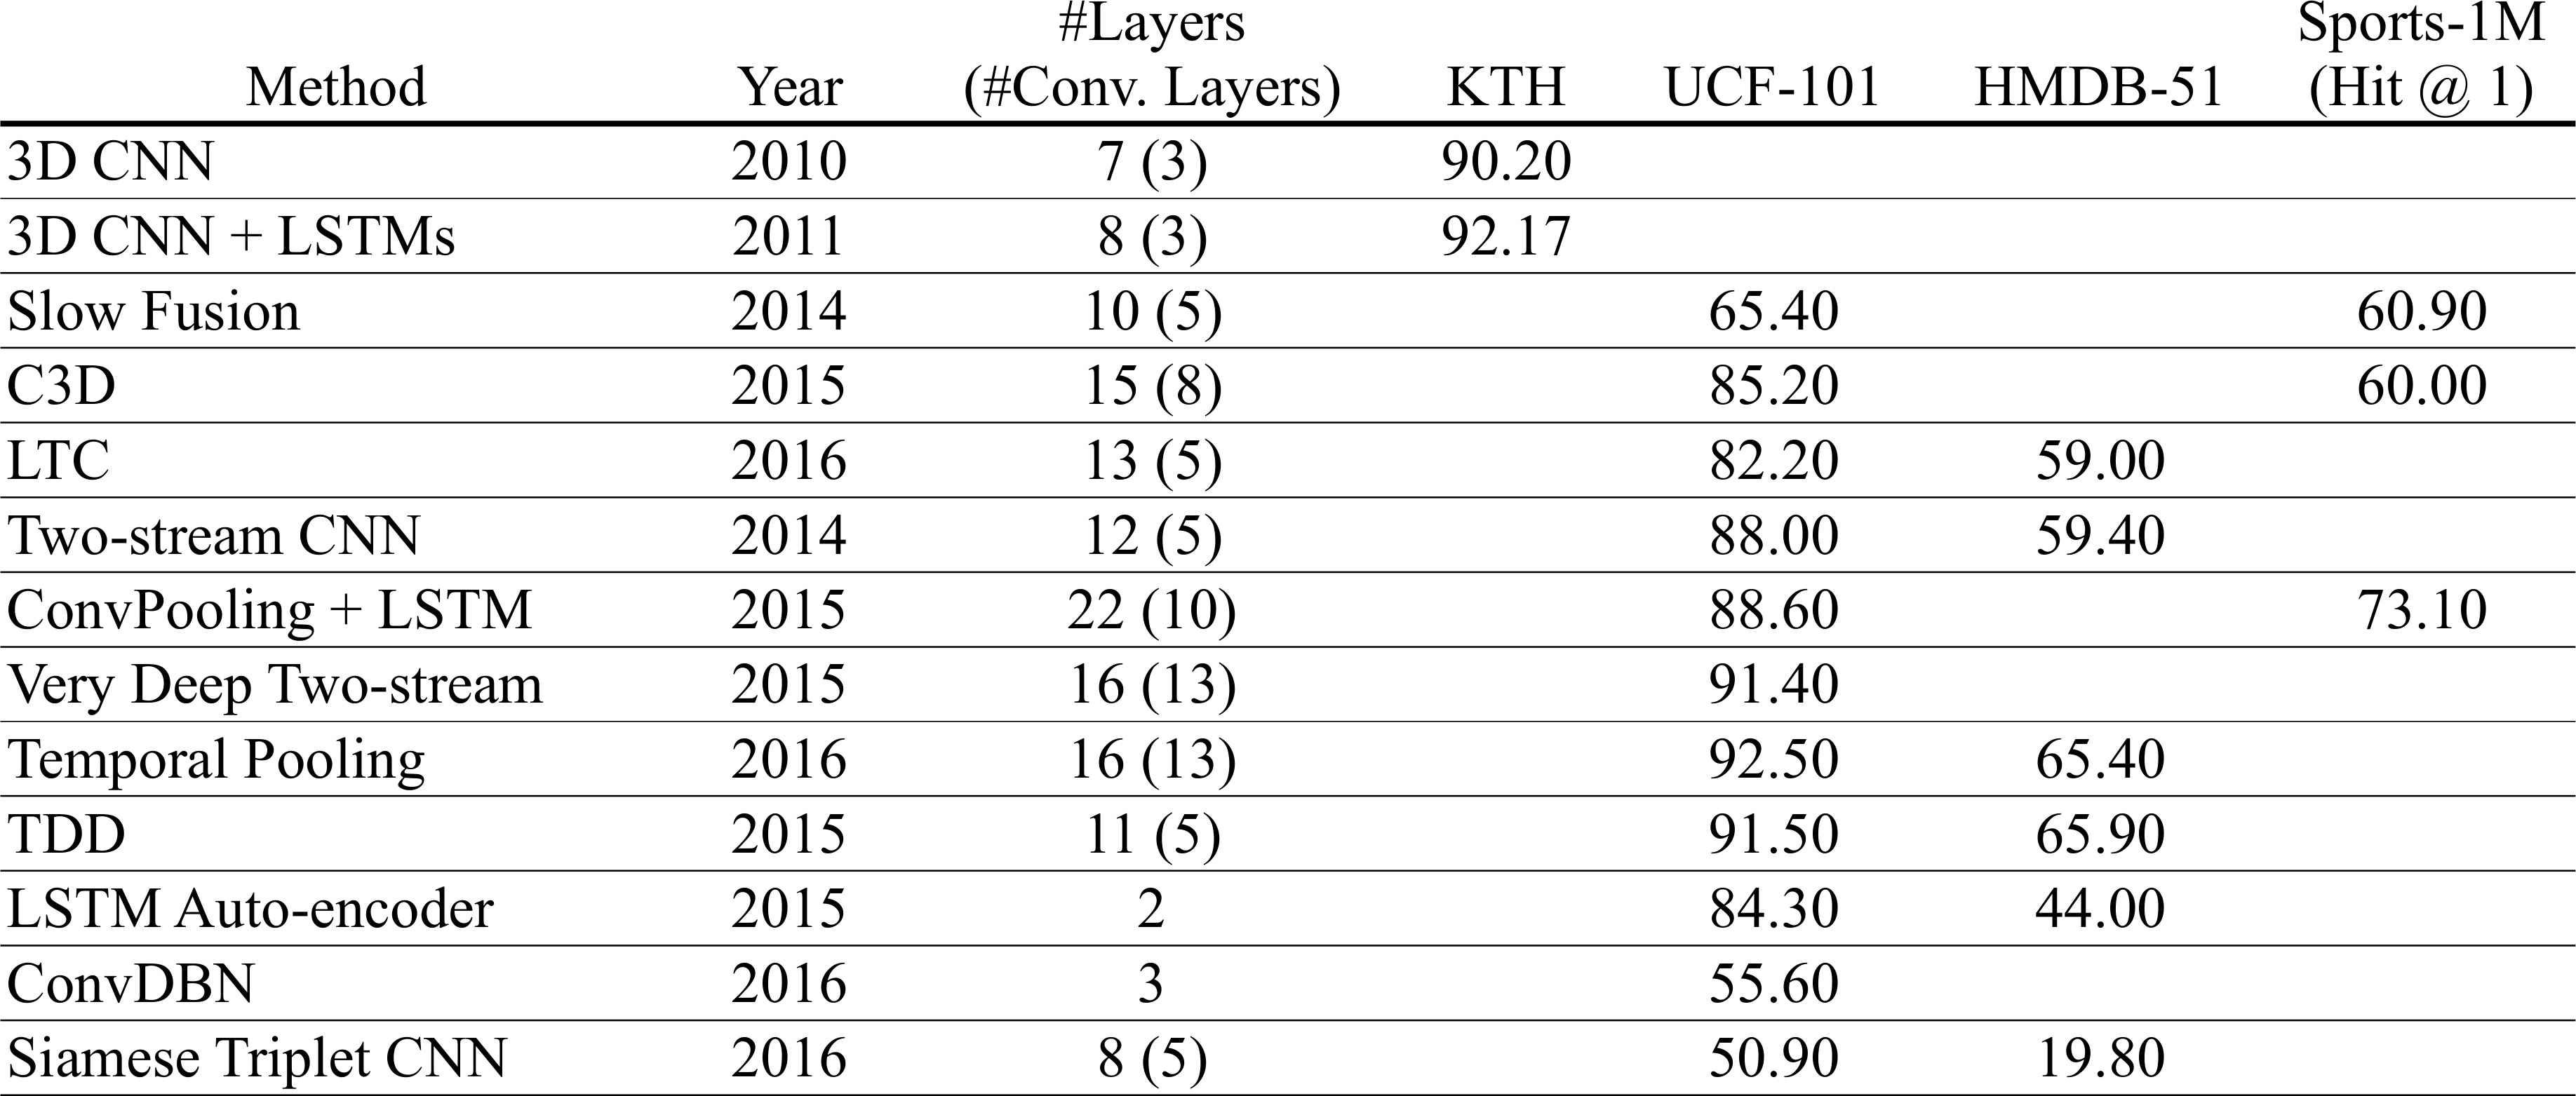
\includegraphics[width=\textwidth]{img_evaluation/deep_results}
    \caption{Best reported action recognition accuracies of reviewed deep learning approaches.}
    \label{tab:deep_results}
\end{table}
\end{minipage}

We observe from the distribution of used benchmarking datasets, that UCF-101 and HMDB-51 can be seen as the current de facto standard benchmarks in action recognition, although UCF-101 is considered extremely small \cite{wang_towards_2015}.
Judging by the best performance on UCF-101, the approaches of \textcite{wang_towards_2015}, \textcite{feichtenhofer_convolutional_2016} and \textcite{wang_action_2015} perform best.
These approaches base on 2D convolutional neural network architectures, that were initially designed for image processing tasks and take advantage of pre-training on large-scale image datasets.
\cite{wang_towards_2015} and \cite{feichtenhofer_convolutional_2016} utilise deep ConvNets in an two-stream setup.
\cite{wang_action_2015} apply a hybrid conventional-deep approach by using a two-stream ConvNet as generic feature extractor along densely sampled trajectories.

Among the approaches, which explicitly incorporate the spatio-temporal structure of videos in the used architecture by implementing 3D convolutions, the \textit{C3D} approach of \textcite{tran_learning_2015} performs best.
\textcite{tran_learning_2015} use a 3D ConvNet which is deeper than comparable approaches (three additional convolutional layers) and leverage pre-training on the Sports-1M dataset.
Since \textit{C3D} is designed for reusability on different vision tasks, an implementation was made publicly available in the Caffe framework \cite{jia_caffe:_2014}.

Given these results it can be derived, that deeper architectures and bigger datasets improve performance in action recognition from video using deep learning approaches.
This has also been observed in the area of object recognition from still images \cite{simonyan_very_2014, szegedy_going_2015, he_deep_2015}.

Table \ref{tab:conventional_results} shows the performance of state-of-the-art hand-crafted feature methods in action recognition.

\begin{minipage}[b]{.03\linewidth}
\setstretch{1.3}
\scriptsize
\cite{wang_action_2013}\\
\cite{wang_action_2013}\\
\cite{cai_multi-view_2014}\\
\cite{lan_beyond_2015}\\
\\
\end{minipage}
\begin{minipage}[b]{.96\linewidth}
\begin{table}[H]
    \centering
    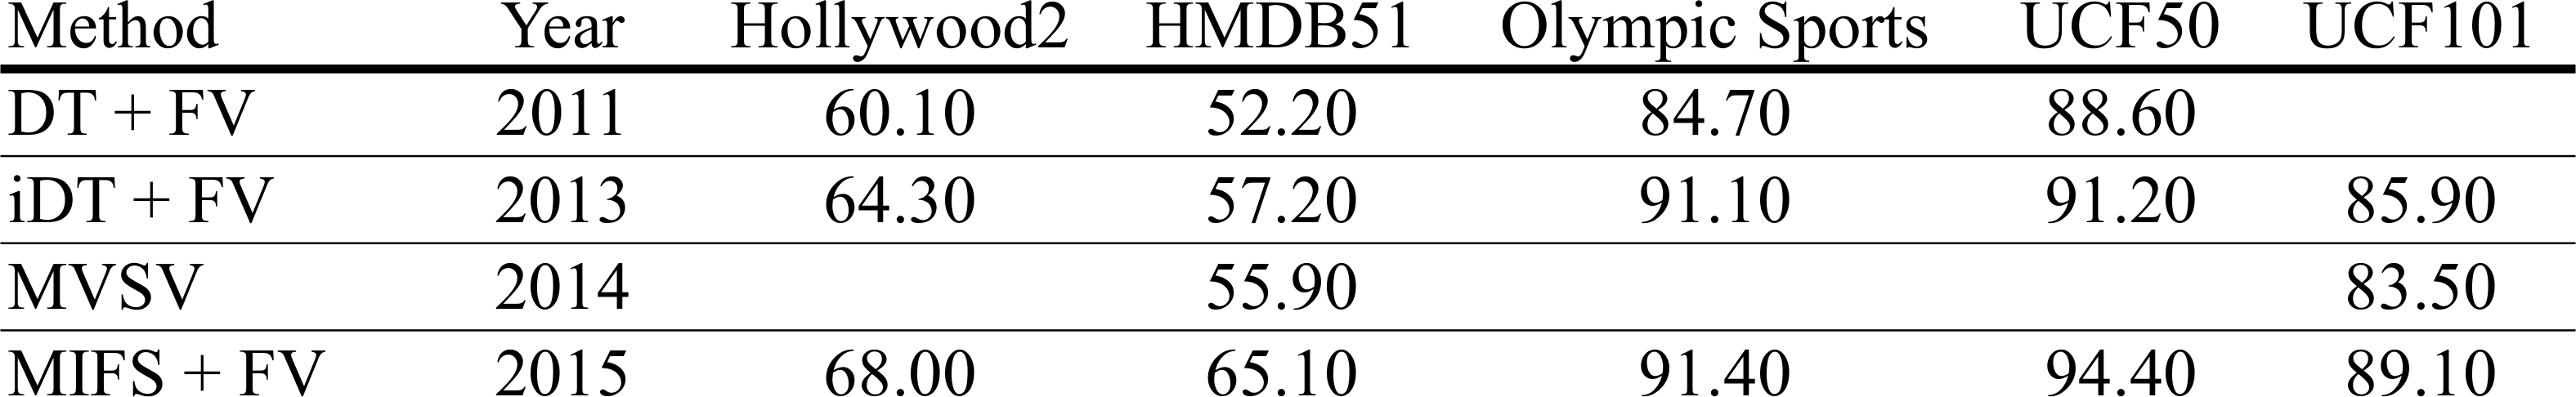
\includegraphics[width=\textwidth]{img_evaluation/conventional_results}
    \caption{Action recognition accuracies of state-of-the-art hand-crafted feature methods.}
    \label{tab:conventional_results}
\end{table}
\end{minipage}

The results on UCF-101 show: Although several deep learning based approaches outperform conventional hand-crafted feature methods, the latter nonetheless yield competitive results, especially the approach of \textcite{lan_beyond_2015}.
Reasons for this can be found in the sizes of available action recognition video datasets.
Table \ref{tab:benchmarks_results} provides a comparison of currently available datasets.

\begin{table}[H]
    \centering
    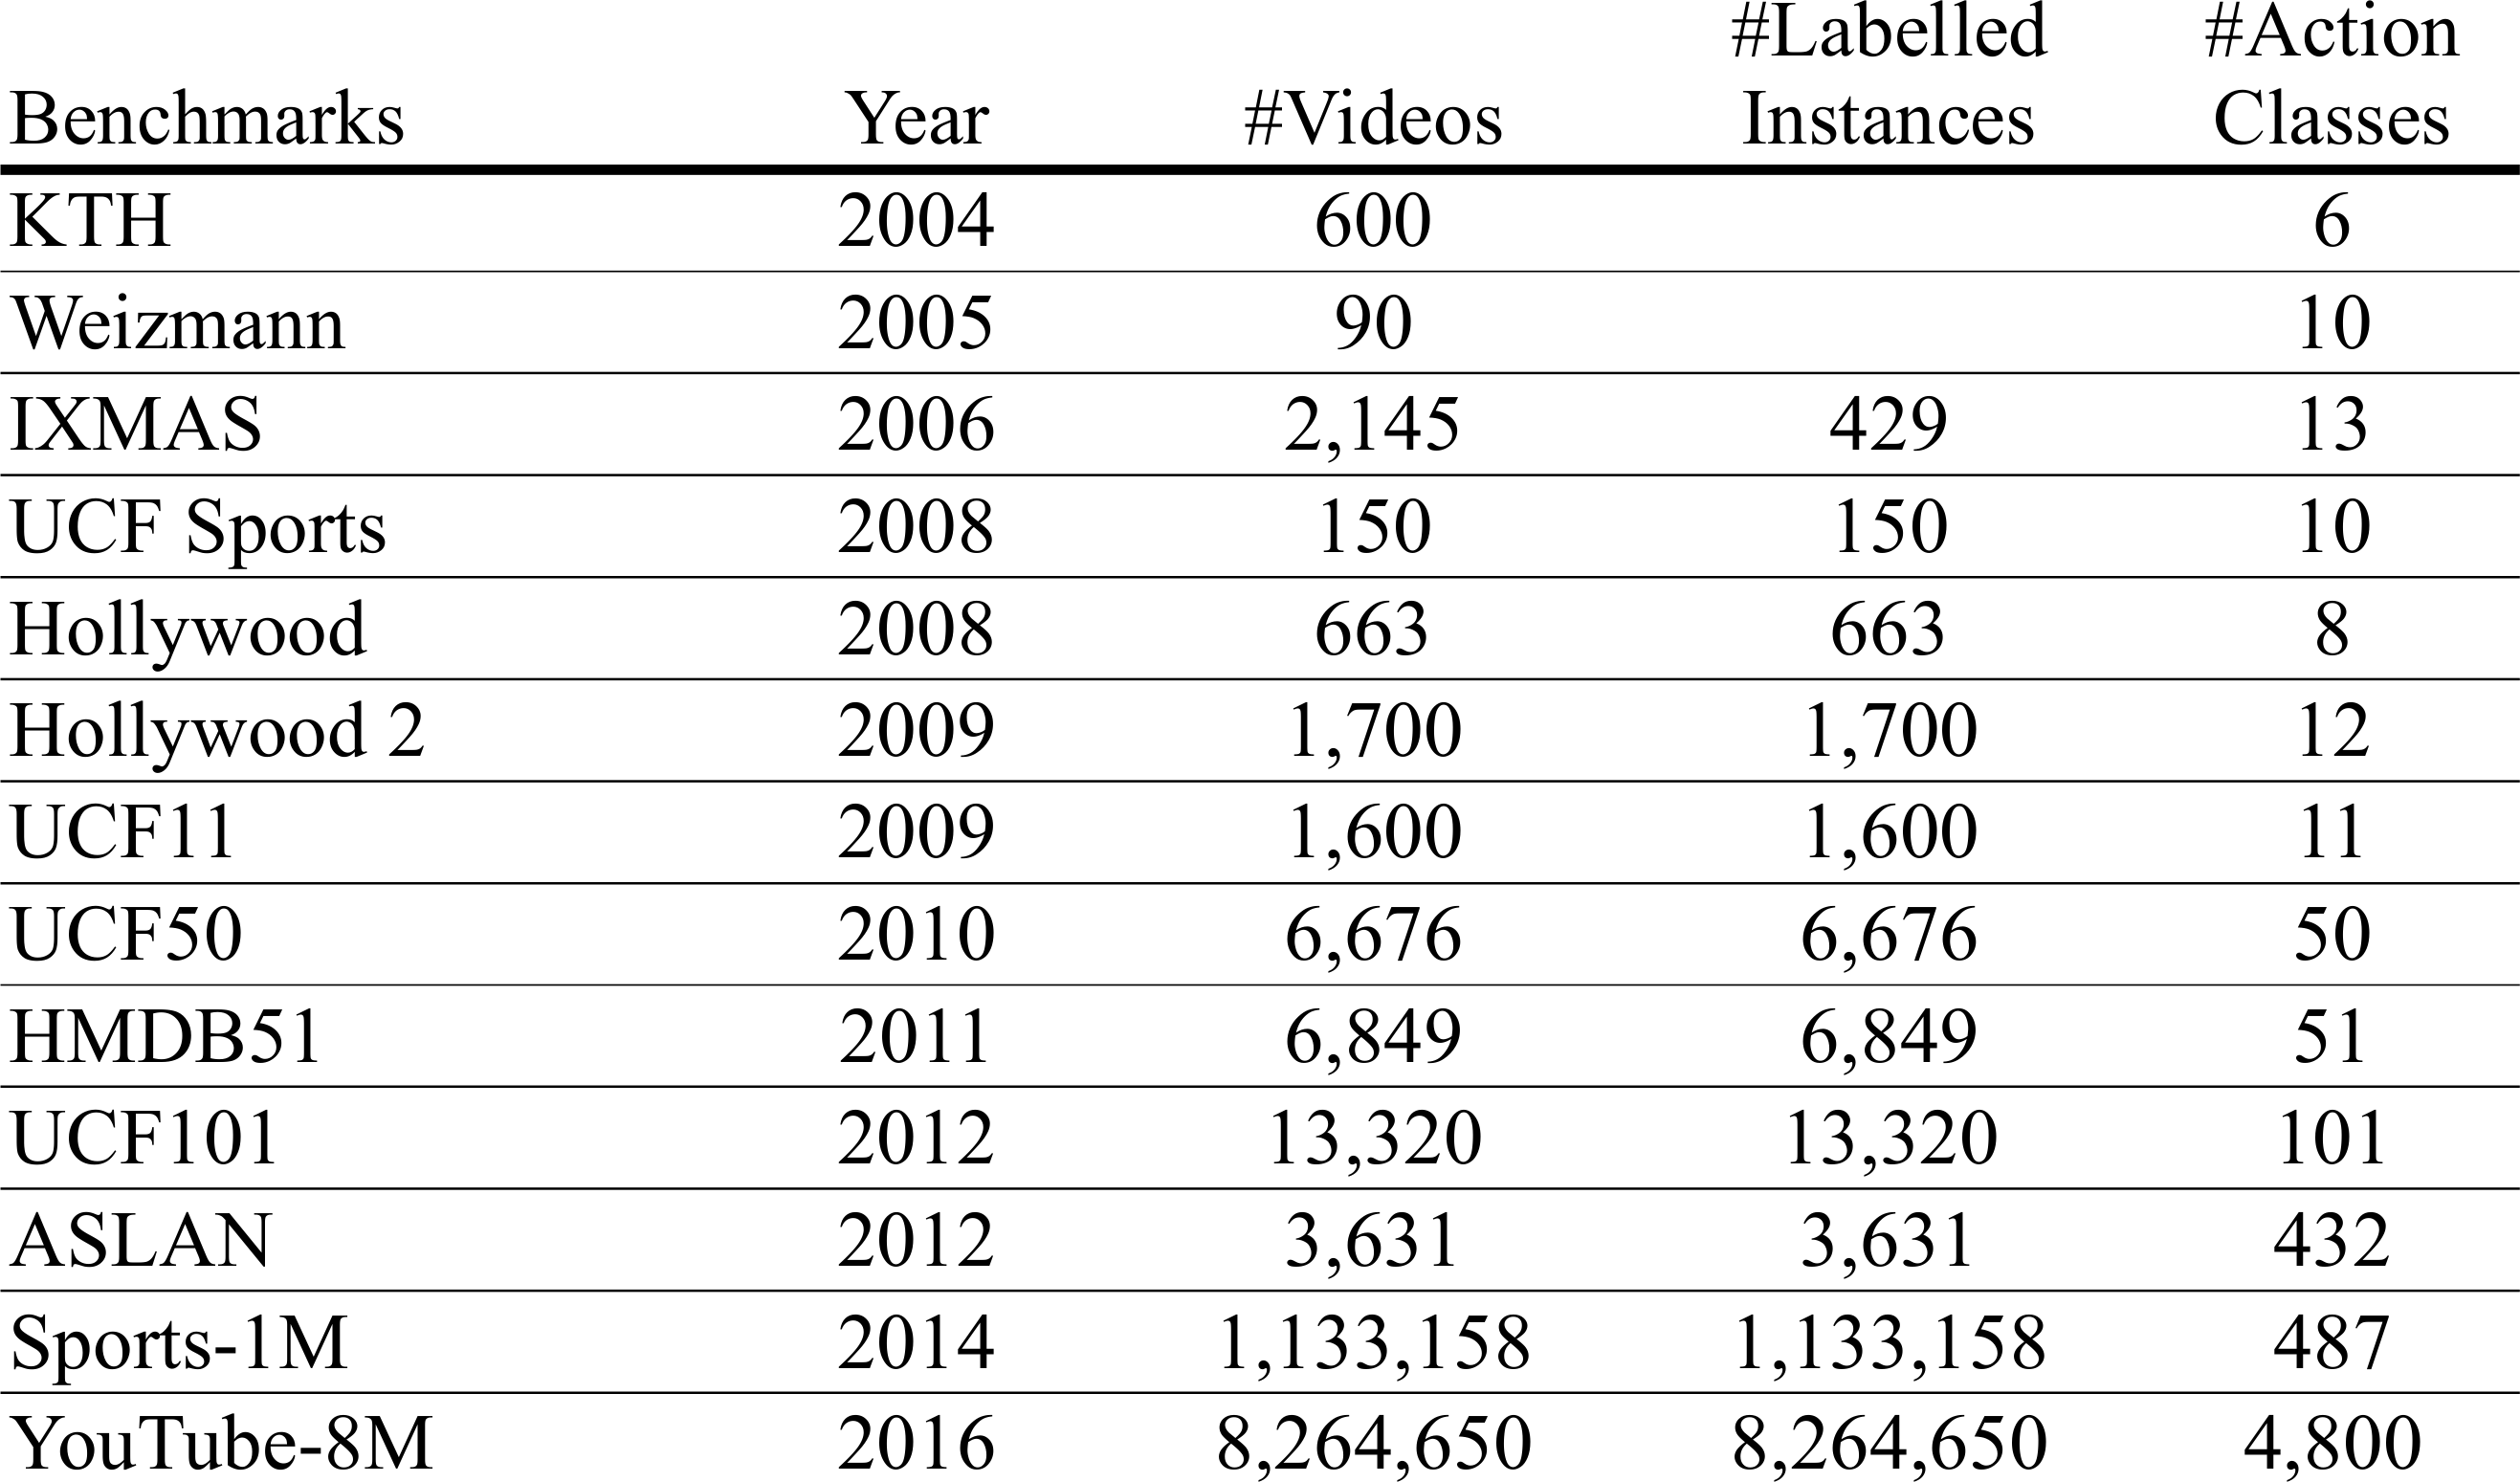
\includegraphics[width=0.7\textwidth]{img_evaluation/benchmarks_results}
    \caption{Size comparison of reviewed benchmarking datasets.}
    \label{tab:benchmarks_results}
\end{table}

Although the Sports-1M dataset is roughly 100 times bigger than UCF101, most approaches rely on the smaller UCF101 or HMDB51 for action recognition, because of the label noise in YouTube-1M \cite{feichtenhofer_convolutional_2016}.
There is a noticeable trend towards larger datasets however.
The very recently released YouTube-8M dataset is roughly eight times bigger than YouTube-1M, but still does not match the size of common image datasets (ImageNet contains $14,197,122$ images \cite{_imagenet_????})
The difficulty to obtain large-scale video datasets originates in videos being more difficult to store and annotate than images \cite{karpathy_large-scale_2014}.

Given its recency, the YouTube-8M has not been used widely in the action recognition community.
Considering its unmatched size in video datasets so far, the creators of the set note, that it will most likely improve the performance of deep learning approaches in action recognition \cite{abu-el-haija_youtube-8m:_2016}.

Table \ref{tab:adl_results} summarizes the characteristics of currently available datasets, that contain videos of the daily-living.

\begin{table}[H]
    \centering
    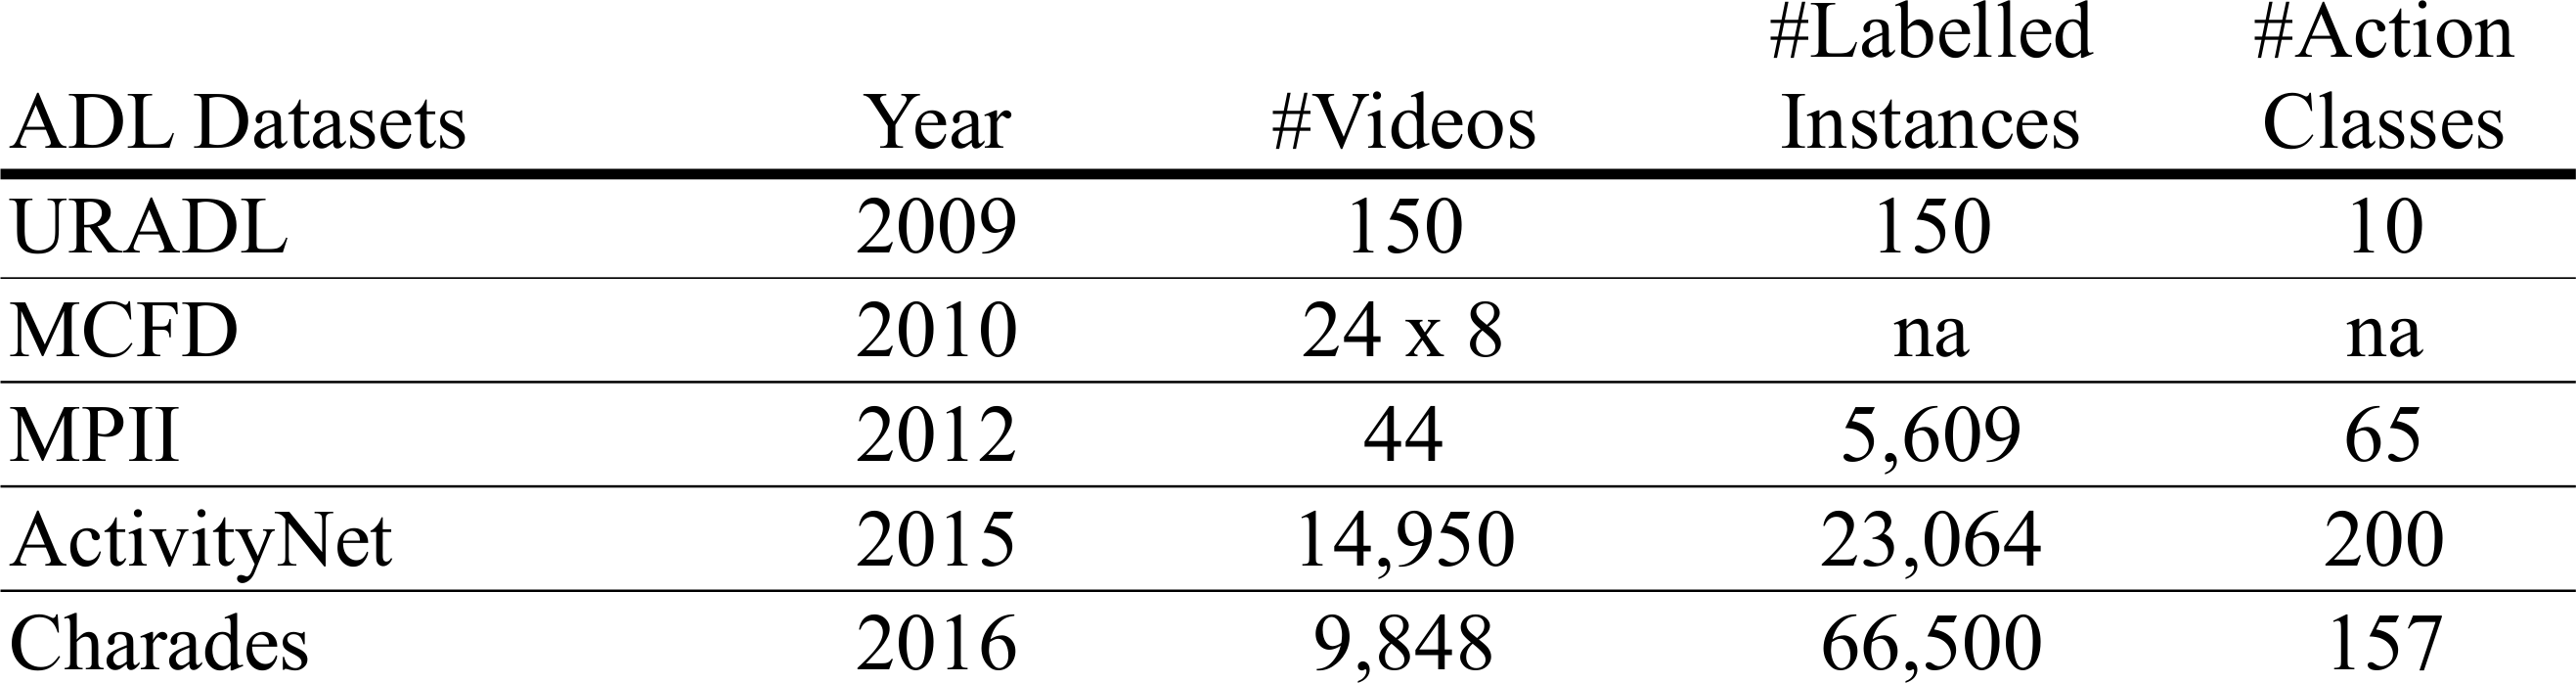
\includegraphics[width=0.7\textwidth]{img_evaluation/adl_results}
    \caption{Size comparison of reviewed daily-living datasets.}
    \label{tab:adl_results}
\end{table}

The Charades dataset \cite{sigurdsson_hollywood_2016} and ActivityNet \cite{caba_heilbron_activitynet:_2015} provide comparably large collections of ADL videos.
Especially the Charades dataset has the advantage of containing videos, that were collected in real-world environments by regular people.
In order to implement an action recognition system in an assisted living environment, we recommend applying the \textit{C3D} approach \cite{tran_learning_2015} to one or possibly both of these datasets.
The advantages of \textit{C3D} are:
\begin{enumerate}
    \item It is the deepest model implementing 3D convolutions.
    \item A model pre-trained on Sports-1M is publicly available.
    \item It was designed to be repurposed on different vision tasks.
\end{enumerate}

\newpage
\section{Conclusion and Future Directions}
This report provides a detailed review of current deep learning approaches in human action recognition from video along with a comparison to conventional hand-crafted feature based approaches.
Results show, that deep learning yields state of the art performance, but conventional hand-crafted feature based methods still perform competitive.
This has been observed in the action recognition community as well \cite{varol_long-term_2016}.

Two reasons for this phenomenon can be identified:
\begin{enumerate}
    \item Current deep learning architectures in video action recognition are shallow compared to their image based counterparts \cite{wang_towards_2015}, because videos are higher dimensional than images and processing them is computationally more expensive.
    \item Available action recognition datasets are too small, since videos are more difficult to store and annotate than images \cite{karpathy_large-scale_2014}\cite{simonyan_two-stream_2014}\cite{wang_towards_2015}
\end{enumerate}

Considering the challenge of obtaining sufficient training data for deep learning architectures, approaches that leverage data from more than one dataset can be identified as future directions of research:
\begin{itemize}
    \item \textbf{Unsupervised Pre-training} as presented in section \ref{sec:generative} of this report and \textcite{varol_long-term_2016}.
    \item \textbf{Transfer Learning} was conducted by \textcite{karpathy_large-scale_2014}.
    \item \textbf{Multi-task Learning} as implemented by \textcite{simonyan_two-stream_2014}.
\end{itemize}

%\subsubsection{Transfer learning}

%See Karparthy 'Large-scale video classification with convolutional neural networks' 2014

%A. S. Razavian, H. Azizpour, J. Sullivan, and S. Carls-
%son. CNN features off-the-shelf: an astounding baseline for
%recognition

%N. Zhang, M. Paluri, M. Ranzato, T. Darrell, and L. Bourdev. Panda: Pose aligned networks for deep attribute modeling. In CVPR, 2014.
%
%B. Zhou, A. Lapedriza, J. Xiao, A. Torralba, and A. Oliva. Learning deep features for scene recognition using places database. In NIPS, 2014.
